\chapter{Midterm 1}
\section{Problem Description and Problem Analysis}
Markup language for interactive storytelling is a relatively new area of focus in the field of digital storytelling. The traditional narrative structure of linear storytelling is being challenged by the emergence of interactive storytelling, which allows the reader to participate in the story and influence its outcome. Markup languages are being developed to facilitate the creation and dissemination of interactive stories.
The problem with traditional linear storytelling is that it does not allow for much interaction from the reader. While the story may be entertaining, it can quickly become predictable and repetitive. Interactive storytelling, on the other hand, allows for the reader to be an active participant in the story, making choices and influencing the outcome.
 However, creating an interactive story can be a complex and time-consuming process. The story must be designed to allow for multiple paths and outcomes, and the technology used to create the story must be able to handle the complexity of the interactive elements. This is where markup languages come in.
Markup languages for interactive storytelling provide a way to structure the story in a way that allows for interactivity. These languages allow for the creation of branching paths, where the reader can make choices that affect the outcome of the story. They also allow for the creation of multimedia elements, such as sound, images, and video, to enhance the storytelling experience.
However, there are several challenges to developing markup languages for interactive storytelling. One challenge is ensuring that the language is easy to use and accessible to both experienced and novice storytellers. Another challenge is ensuring that the language is flexible enough to allow for a wide range of storytelling styles and genres.
In the end, the development of markup languages for interactive storytelling is an exciting area of innovation in the world of digital storytelling. As the technology continues to develop, we can expect to see more and more interactive stories being created and shared, providing readers with a more engaging and immersive storytelling experience.

What is the solution concept?

To address the need of creation of a markup language for story-telling the demand for which has surged in the past decade with popularization of visual novels, one can be developed from scratch, the goals of such language would be to provide authors with a toolset for creating engaging interactive stories that are easily shared and played by the audience.

The first step in developing is identifying the key elements that make up an interactive narrative. At high level such a story consists of a series of scenes or chapters that the player progresses through, with each scene offering a set of choices that can affect the story’s outcome. Therefore, the language must be capable of representing these elements, be easily understandable and machine readable.
One possible solution is to use XML-based format, with each scene represented as an individual element within the document. These scenes can be further broken down into sub-elements that represent the various narrative components, such as dialogue, actions and character descriptions. Similarly, the choices that the player makes can be represented as elements within each scene, with the outcome of each choice encoded as an attribute of that element.

To ensure that the language is both human-readable and machine-readable, it may be helpful to include annotations or comments within the markup. These annotations can help authors understand the structure and flow of the story, while also providing hints for how to use various elements and attributes. Additionally, including metadata such as the author's name and the date of creation can help to track the ownership and history of the story.

Once the basic structure of the markup language has been established, the next step is to define a set of rules for how the language should be used. This can include guidelines for naming conventions, data types, and formatting, as well as rules for how the language should be validated and parsed.

To ensure that the markup language is user-friendly, it may be useful to provide a set of tools or templates that authors can use to create and edit their stories. These tools could include a graphical user interface for creating and editing scenes, as well as a validator that checks the markup for errors and inconsistencies. Additionally, providing a set of pre-built components or templates that authors can use as a starting point for their stories can help to speed up the development process and ensure consistency across different stories.

One possible example of a successful markup language for interactive storytelling is Inkle's Ink software. Ink is a powerful, flexible language that allows authors to create complex, branching narratives with ease. It features a robust set of tools for editing and testing stories, as well as a built-in interpreter that can be used to play the stories on a variety of platforms. In creating our own markup language the strive would be to mimic with possible improvements the feature set of Inkle’s solution on interactive storytelling writing.

 What is the impact of the problem over the domain of study?

 Interactive storytelling programming languages, or ISPLs, are programming languages designed specifically for the creation of interactive narratives and games. These languages offer a unique and powerful tool for creating immersive and engaging experiences for users. The impact of ISPLs on the programming domain can be significant in several ways:

 \begin{enumerate}
                 \item Increased creativity: ISPLs offer a new way for programmers to express their creativity. With ISPLs, programmers can use their skills to create engaging narratives, characters, and interactive elements that keep users engaged and interested in the story. This can be a refreshing break from traditional programming, which often involves working on utilitarian projects.
                 \item Expansion of the programming domain: ISPLs can attract a new group of programmers who are interested in creating interactive stories and games. This can expand the programming domain and attract new talent to the industry. Additionally, ISPLs can allow developers to create new types of programs and applications that were not possible before, such as interactive educational tools, immersive simulations, and more.
                 \item Enhanced user engagement: ISPLs can help developers create interactive stories and games that are more engaging and immersive for users. By combining storytelling with programming, developers can create experiences that are more engaging than traditional software. This can be especially useful for educational tools, which can use interactive narratives to teach complex concepts in a more engaging way.
                 \item Improved user experience: ISPLs can help developers create applications with a more natural user interface. With interactive storytelling, users can navigate through the application in a more intuitive way, using conversation or exploration, which can lead to a better overall user experience.
 \end{enumerate}
 Overall, ISPLs have the potential to be a powerful tool for programmers, allowing them to create engaging interactive narratives and games that can expand the programming domain and offer users more engaging and immersive experiences.

 What are the Competition and Alternatives?

 \begin{itemize}
                \item \textbf{Inky}
 \end{itemize}
 
Inky is a free, open-source tool designed to create interactive narrative scripts for video games. It is primarily used in the development of games that use the ink narrative scripting language, which was created by the game development studio, Inkle.
Inky is designed to make it easier for writers and developers to create and iterate on interactive narrative content without the need for programming expertise. It provides a user-friendly interface where writers can easily create, edit, and preview ink scripts. Inky also provides tools for managing branching paths, variables, and game logic.
In addition to its editing capabilities, Inky also provides features for version control, collaboration, and integration with game engines. It can output ink scripts in a variety of formats, including JSON, XML, and custom C# classes.
Overall, Inky is a powerful and flexible tool for creating interactive narratives for games, enabling writers and developers to work more efficiently and collaboratively in the creation of immersive game experiences.
\begin{itemize}
                \item \textbf{Yarn Spinner}
 \end{itemize}
 
 Yarn Spinner is an open-source tool designed to help game developers and writers create branching, non-linear narratives for video games. It was created by the game development studio, Secret Lab, and is free to use under the MIT license.
Yarn Spinner uses a scripting language called Yarn, which is designed to be easy to read and write, and allows writers to create complex branching paths and dialogue trees for their game's characters. The Yarn language is similar in structure to a simplified version of JavaScript, making it easy for developers with some programming experience to use.
In addition to its scripting capabilities, Yarn Spinner also includes a powerful dialogue engine that can handle complex conversations, conditional branching, and other advanced features. It can be integrated with various game engines, including Unity, Unreal Engine, and Godot.
Yarn Spinner also includes a number of features to help developers and writers collaborate on game narrative. It allows multiple writers to work on the same project simultaneously, provides version control, and includes a number of debugging and testing tools.
Overall, Yarn Spinner is a powerful and flexible tool for creating interactive narratives for video games, making it easier for developers and writers to create immersive, non-linear stories that engage players and keep them coming back for more.

 \begin{itemize}
                \item \textbf{StoryMapJS}
 \end{itemize}

 StoryMapJS is a free, open-source tool that allows users to create interactive maps with multimedia content, such as images, videos, and audio. It was created by the Knight Lab at Northwestern University and is designed to help journalists, educators, and others tell stories in an engaging and visually compelling way.
With StoryMapJS, users can create a sequence of locations on a map, and add multimedia content to each location. This can include images, videos, audio, and text. Users can also add annotations, captions, and other information to provide context and guide readers through the narrative.
StoryMapJS provides a simple, user-friendly interface for creating these interactive maps, and can be used by anyone with basic web development skills. The resulting map can be embedded on a website or shared as a standalone link, making it easy to distribute and share with others.
Overall, StoryMapJS is a powerful and flexible tool for creating interactive maps with multimedia content. It is ideal for educators, journalists, and others who want to tell stories in an engaging and visually compelling way, and can be used for a wide range of applications, from historical tours to travel guides to news stories.

Who is the Target audience?

A target audience is a group of people that are most likely to be interested in our service or product. The target group for interactive storytelling can vary on the specific story, format, genre or way of implementation. However, interactive storytelling is often designed for people who are ready to engage completely in the action, and be allowed to participate in the storyline, rather than just passively consuming it.
Some examples of target groups for interactive storytelling might be:

 \begin{enumerate}
                 \item Children and young adults: Interactive storytelling can be a fun and educational way to engage younger audiences and get them excited about reading and storytelling. Many interactive storybooks and apps are designed with children in mind, using interactive elements like animation and sound effects to make the story come to life.
                 \item Adults: Even for mature people, this could be an interesting way of entertainment. As many people are into reading books, some of them would be more than happy to be able to influence the development of the story.
                 \item Gamers: Interactive storytelling is often a key component of video games, which can appeal to a wide range of ages and interests. Games that feature branching narratives, player choices, and other interactive elements are particularly popular among gamers who enjoy engaging storytelling experiences.
                 \item Virtual reality enthusiasts: Virtual reality (VR) technology allows users to step into and interact with immersive digital environments, making it a perfect medium for interactive storytelling. VR experiences can be particularly appealing to well-informed people in the use of modern technology, who are looking for new and innovative ways to engage with stories.
 \end{enumerate}

 To sum up, the target group for interactive storytelling can be quite broad, and may appeal to anyone who is looking for a more immersive and interactive way to experience stories where it will be possible to influence the development of the storyline.

 What is our Motivation?
 
As a group of students who are passionate about computer science and storytelling, we have identified a gap in the current programming languages available that cater specifically to interactive storytelling. While there are many programming languages out there that allow users to create games or simulations, these languages don't always make it easy to create interactive stories that have branching paths and multiple endings.                                                    
We believe that interactive storytelling is a powerful tool for teaching and entertainment, and we want to make it more accessible to people who are interested in this field. We are motivated to develop a programming language that makes it easy for people to create interactive stories, regardless of their level of programming expertise.
We want to create a language that is intuitive, user-friendly, and flexible. It should allow users to easily create branching story paths, define character actions and dialogue, and create different outcomes based on user input. This language should also be easy to learn, so that even people who have no experience with programming can use it to create compelling interactive stories.
We are motivated to create this language because we believe that interactive storytelling has the potential to be a powerful educational tool. It can help students learn important concepts by engaging them in a narrative that allows them to explore different scenarios and outcomes. By making interactive storytelling more accessible, we hope to inspire more people to explore this exciting field and create engaging, interactive stories that can be shared with others.



\addcontentsline{toc}{section}{Implementation plan}
\section{Implementation plan} To have a better view on our Implementation plan let's define for the beggining the domain.
The domain of interactive storytelling encompasses a wide range of creative industries, including gaming, film, literature, and education. In recent years, there has been a growing demand for more engaging and immersive forms of storytelling, and interactive storytelling has emerged as a popular solution to this demand. Interactive storytelling allows readers to participate in the story and influence its outcome, providing a more dynamic and personalized experience.


Moreover, a DSL for interactive storytelling could also facilitate collaboration and knowledge sharing within the domain. Domain experts can share best practices, templates, and tools that could help other creators to design and produce high-quality interactive stories, accelerating the development of the field. A DSL can also provide a standard language and structure for interactive stories, making them easier to share and disseminate across different platforms and devices.

In addition to the benefits mentioned earlier, a DSL for interactive storytelling could also enable domain experts to create more sophisticated and complex narratives. Currently, most interactive stories are limited in their complexity due to the technical skills required to program them. A DSL for interactive storytelling could provide an accessible platform for creators to design and produce stories with more intricate plot lines, character interactions, and decision trees.

Another benefit of a DSL for interactive storytelling is that it could help bridge the gap between the creative and technical aspects of interactive storytelling. Often, domain experts are required to collaborate with technical experts to develop interactive stories, which can be a time-consuming and challenging process. A DSL for interactive storytelling that is designed to be user-friendly and accessible to non-technical experts could enable domain experts to take a more hands-on role in the development process, reducing the need for technical support.
Furthermore, a DSL for interactive storytelling could help streamline the production process for interactive stories. Currently, creators often have to rely on different software tools and platforms to create and publish their interactive stories, which can be a cumbersome and inefficient process. A DSL for interactive storytelling that offers a complete set of tools and functionalities could simplify the production process and reduce the time and effort required to produce high-quality interactive stories.

The problem being addressed is the creation of a DSL that provides a more intuitive and concise way to create interactive stories. While there are numerous programming languages available for developing games and simulations, these languages don’t always make it simple to create interactive stories with different pathways and multiple outcomes. There were implemented several tools for operating with narrative text, for example Inky editor [2].	
These types of languages are used by people who like to engage in action completely, so the aim is to please different groups of people, including: young adults, gamers and virtual reality enthusiasts. It should allow users to easily create branching story paths, define character actions, dialogue, and create different outcomes based on user input. This language should also be easy to learn, so that even people who have no experience with programming can use it to create compelling interactive stories.


Overall, a DSL for interactive storytelling has the potential to revolutionize the way we create and consume stories, making them more engaging, immersive, and accessible to a wider audience. By providing a standardized language and structure for interactive stories, a DSL can also help to establish interactive storytelling as a recognized and respected art form, opening up new opportunities for domain experts in a rapidly growing field.

In summary, the development of a DSL for interactive storytelling can benefit domain experts by simplifying the process of designing and producing interactive stories, promoting collaboration and knowledge sharing, and standardizing the language and structure of interactive stories.

\textbf{What is the basic computation that the DSL performs (i.e., what is the computational model)?}

The imperative model would be used to define the sequence of events that occur in the story, and to specify the conditions that must be met for certain events to take place. This would include specifying the order in which story segments are displayed or activated, as well as specifying the options and choices available to the reader at various points in the story.
The declarative model would be used to define the characters, settings, and objects in the story, as well as the relationships and interactions between them. This would include specifying the various attributes and properties of characters and objects, such as their personalities, abilities, and status, as well as the constraints and requirements for different story paths and endings.

The language might also incorporate elements of a functional model, as it may need to process and manipulate data (such as the reader's choices or the state of the story) to determine the next steps in the narrative.

\textbf {What are the basic data structures in your DSL? How does a the user create and manipulate data?}

The basic data structures are likely to include objects, variables, and collections. These data structures are used to represent characters, settings, objects, and events in the story, as well as to store and manipulate data throughout the narrative.

Objects: Objects are the fundamental building blocks of your DSL's data structures. In Inky, objects are used to represent characters, settings, and objects in the story, as well as to define their attributes and properties. The user can create and manipulate objects using simple and intuitive syntax, such as defining an object's name, description, and relationships with other story elements.

Variables: Variables are used to store and manipulate data in your DSL. Variables can be used to store the state of the story, such as the reader's choices and the current location in the narrative. The user can create and manipulate variables using simple syntax, such as assigning a value to a variable or retrieving its current value.

Collections: Collections are used to group related data together in your DSL. Collections can be used to represent lists of objects, such as a list of characters in the story or a list of possible story paths based on the reader's choices. The user can create and manipulate collections using simple syntax, such as adding or removing objects from a collection or iterating over its contents.

To create and manipulate data in our DSL, the user would typically use a combination of declarative and imperative syntax. The declarative syntax is used to define the structure and content of the story, including the objects, variables, and collections that will be used to represent and manipulate data. The imperative syntax is used to control the flow of the narrative and to manipulate data based on the reader's choices and actions.

For example, the user might define a collection of possible story paths based on the reader's choices, and then use imperative syntax to evaluate the reader's current choice and determine which path to follow. The user might also define a variable to represent the reader's current location in the story, and then use imperative syntax to update the variable as the story progresses.

\textbf {What are the basic control structures in your DSL? How does the user specify or manipulate control flow?}

In our DSL for interactive storytelling, the basic control structures are likely to include branching and looping structures. These control structures are used to control the flow of the narrative based on the reader's choices and actions.

Branching Structures: Branching structures are used to control the flow of the narrative based on conditional logic. In our DSL, the user can use branching structures to evaluate the reader's choices and actions, and then determine which story path to follow. This can be done using simple syntax, such as an "if" statement that checks the value of a variable and then executes different actions based on the result. For example, the user might use an "if" statement to evaluate the reader's choice and then branch to different story paths depending on which option was chosen.

Looping Structures: Looping structures are used to repeat a set of actions multiple times. In our DSL, the user can use looping structures to create repeating elements in the story, such as a character performing a series of actions or the reader revisiting a location multiple times. This can be done using simple syntax, such as a "while" or "for" loop that executes a set of actions repeatedly until a condition is met. For example, the user might use a "while" loop to repeat a set of actions until a certain event occurs, such as the reader finding a key or completing a puzzle.

The user can specify and manipulate control flow in our DSL using a combination of declarative and imperative syntax. The declarative syntax is used to define the structure and content of the story, including the branching and looping structures that will be used to control the flow of the narrative. The imperative syntax is used to evaluate the reader's choices and actions, as well as to manipulate data and control flow based on these choices and actions.

For example, the user might define a branching structure to evaluate the reader's choice and determine which story path to follow. The user might also use imperative syntax to manipulate data and control flow based on the reader's choices, such as updating a variable to represent the reader's current location in the story or branching to a different story path based on the outcome of a puzzle or encounter. Overall, the basic control structures in your DSL would allow the user to create engaging and interactive narratives that can adapt to the reader's choices and actions.

\textbf {What kind(s) of input does a program in your DSL require? What kind(s) of output does a program produce?}

A program or DSL for interactive storytelling would typically require input from the reader in the form of choices, interactions, and other types of user input. This input would be used to control the flow of the narrative and to manipulate data, such as updating the state of the story based on the reader's choices.
Some specific types of input that a program in our DSL might require include:

\begin{itemize}
                \item Reader choices: The reader might be presented with a set of options, such as dialogue choices or actions to take, and then select one of these options to continue the story.
                \item Interactions: The reader might interact with elements of the story, such as clicking on an object or navigating to a new location, and then trigger a new set of actions or dialogue.
                \item Puzzle or game elements: The reader might need to solve puzzles or complete challenges in order to progress through the story, requiring specific input such as text inputs or clicking on certain elements.
 \end{itemize}
A program in our DSL would produce output in the form of the narrative text and visual elements that are displayed to the reader, as well as updates to the state of the story based on the reader's choices and actions. The specific types of output that a program in our DSL produces might include:

\begin{itemize}
                \item Narrative text: This is the core output of the program, consisting of the text that describes the story, characters, and events.
                \item Visual elements: The program might also produce visual elements to enhance the story, such as images, videos, or animations.
                \item Sound or music: The program might incorporate sound or music to enhance the mood or atmosphere of the story.
                \item Updates to the state of the story: As the reader progresses through the story and makes choices or takes actions, the program would produce updates to the state of the story, such as changing the current location or updating the inventory of the reader's character.
 \end{itemize}

\textbf {Error handling: How might programs go wrong, and how might  language communicate those errors to the user?}

In a DSL for interactive storytelling, there are several ways that programs might go wrong. Here are some examples:
\begin{itemize}
                \item Data errors: when the program manipulates data in unexpected ways, such as by accessing data that has not been initialized or by trying to perform an operation on incompatible data types.
                \item Logic errors: Logic errors occur when the program's code does not correctly reflect the intended logic of the story. For example, a branching structure might not accurately evaluate the reader's choices or a loop might not correctly repeat the desired actions.
 \end{itemize}
When programs encounter errors, it is important to communicate these errors to the user in a clear and understandable way. Here are some ways that a DSL might communicate errors to the user:
\begin{itemize}
                \item Error messages: The program might display an error message to the user, explaining what went wrong and how to fix it. This could include specific details about the error, such as which line of code caused the error or which input was invalid.
                \item Debugging tools: The DSL might provide debugging tools to help the user identify and fix errors. This could include features like step-through debugging, where the user can step through the code line-by-line and inspect the values of variables and data structures.
 \end{itemize}
 
\textbf {Are there any other DSLs for this domain? If so, what are they, and how will your language compare to these other languages?} 

Yes, there are other DSLs for interactive storytelling. Here are a few examples:
 \begin{enumerate}
                 \item Twine: Twine is a popular open-source tool for creating interactive stories. It uses a visual interface to allow authors to create branching stories and add multimedia elements. Twine supports a variety of export formats, including HTML, CSS, and JavaScript.
                 \item ChoiceScript: ChoiceScript is a DSL developed by Choice of Games, a company that specializes in creating interactive fiction. It uses a text-based scripting language to allow authors to create branching stories with variables and conditionals. The company also provides a publishing platform for authors to distribute their games.
                 \item Ren'Py: Ren'Py is a DSL specifically designed for creating visual novels, a sub-genre of interactive fiction. It uses a Python-based scripting language to allow authors to create branching stories with custom UI elements, sound, and music. Ren'Py also provides a publishing platform for authors to distribute their games.
                 \item Inky:Compared to these other DSLs, Inky focuses on providing a simple and intuitive way for authors to create branching stories using a plain text format. It is designed to be easy to learn and use, with a minimal syntax and support for inline comments and documentation. Inky also provides support for exporting stories to a variety of platforms, including HTML, JSON, and InkJS, which allows the stories to be integrated into websites or other applications.
 \end{enumerate}

\textbf {Here is an overview of our implementation plan:}

\textbf {Define the scope and goals of our language:} Start by defining the scope and goals of your language. Determine what specific features and functionality you want to include and what kind of user experience you want to provide. This will help you prioritize your implementation efforts and focus on the most important aspects of your language. 

\textbf {Choosing a host language:} Decide on a programming language or platform to use as the host for your DSL. The host language should be well-suited to the task of sound processing and have the necessary tools and libraries to support your language. 

\textbf {Choosing a parser and interpreter strategy:} Decide on a strategy for parsing and interpreting the code written in your language. You might choose to use an existing parser or build your own, depending on your specific needs and resources. 

\textbf {Designing the syntax and grammar of your language:} Design the syntax and grammar of your language to be clear, consistent, and easy to understand. Use established conventions and patterns to make your language more accessible to users. 

\textbf {Implementing the core features of your language:} Start implementing the core features of your language, such as the ability to load and process audio files, generate and manipulate sound waves, and apply various effects and filters.

\textbf {Testing and debugging your language:} Test and debug your language as you implement new features. Make sure to identify and address any bugs or performance issues as they arise. 
Documenting our language: Document your language to make it easier for users to understand and use. Provide clear instructions and examples to help users get started with your language and troubleshoot common issues. 

\textbf {Refining and improving your language:} Continuously refine and improve your language based on feedback from users and your own experience working with it. Add new features and functionality as needed to make your language more useful and powerful.


\addcontentsline{toc}{section}{Teamwork plan}
\section{Teamwork plan}
When implementing a programming language for interactive storytelling, the tasks can be divided among the team members based on their skills, expertise, and interests.
 \begin{enumerate}
                 \item Design and planning: One team member can lead the design and planning process, which involves defining the language features, syntax, and semantics. 
                 \item Programming language implementation: Another team member can lead the implementation of the programming language. This person should be experienced in programming language implementation, particularly in lexing, parsing, and code generation.
                 \item Editor implementation: A team member can focus on building an editor for the programming language.
                 \item Interactive Storytelling content: A team member can focus on creating the interactive storytelling content, which involves writing the scripts and storylines that use the programming language. This person should be skilled in creative writing and have a good understanding of interactive storytelling.
                 \itemTesting and debugging: One team member can focus on testing and debugging the programming language implementation and editor. 
 \end{enumerate}
It is important to ensure that each team member's tasks are well-defined and aligned with the project's goals. Furthermore, we are determined that each team member will work on every aspect of the project, including research, design, implementation and documentation. 

\addcontentsline{toc}{section}{Grammar}
\section{Grammar}

\noindent For a better understanding, further is represented the grammar for this specific language according to a very simple and textual program. Through it, was shown in detail each feature of grammar.
The DSL design includes several stages. First of all, definition of the programming
language grammar  
G = (VN,VT, P, S ):

VN – is a finite set of non-terminal symbol;

VT - is a finite set of terminal symbols.

P – is a finite set of production of rules;

S - is the start symbol;\\

$VN = {<program>, <var>, <knot>, <ID>, <content>, <text>, <goto>, <print>,$
$<img>, <choice>, <var_op>, <expr>, <int>, <str>, <value>, <var_name>, $
$<knot_name>, <img_name>, <option_text>, <EQ>, <LPAREN>, <RPAREN>, <LCURLY>, $
$<RCURLY>, <GH>, <EXLAM>, <IMG_NAME>, <INT>, <ID>, <WS>, <EOF>} $

$VT = {'EOF', '(', ')', '*', '=', '<', '>', '[', ']', '{', '}', '!', '+', '-', '/', '(', ')(', ')', '<', '>', '=', '[', ']', '!', a'{', '}', ',', $
$'.png', '.jpg', ‘0’..’9’, ‘a..z’, ‘A’..’Z’}$

\noindent In Table 1 are meta-notations used for specifying the grammar. 
\begin{table}[h]
    \centering
    %\caption{Meta notation} C-c
    \begin{tabular}{|c|c|}
        \hline
        Notation (symbol) & Meaning\\
        \cline{1-2}
        $<foo>$ & means foo is a nonterminal\\
        \hline
        foo & foo in bold means foo is a terminal\\
        \hline
        x* & zero or more occurrences of x\\
        \hline
        $|$ & separates alternatives\\
        \hline
        → & derives\\
        \hline
        // & comment section\\
        \hline
    \end{tabular}
    \label{tbl:epochs}
\end{table} \\
\begin{verbatim}
    <program>→ (<var>)* <knot>+ EOF
    
    <knot> → <ID> '{' <content>* '}' 
    <var> → <var_name> '=' <value>
    <value>→ <int>|<str>
    <int>→<INT>
    <str>→'"'(<ID>|<INT>)*'"'
    
    <content>→ <text>
    	| <goto>
    	| <print>
    	| <img>
    	| <choice>
    	| <var_op>
    
    <var_op> : '[' <var_name> '=' <expr> ']'
    
    <expr>:   <expr> ('*'|'/') <expr>
    	|   <expr> ('+'|'-') <expr>
    	|   <int>
    	|   '(' <expr> ')'
    	|   <str>
    	| <var_name>
    
    <goto> → '(' <knot_name> ')' 
    <print> → '(''(' <var_name> ')'')'
    <img> →'(''!' <img_name> ')'
    <choice>→ '(' '(' <pair>*  ')'')'
    <pair>→'!'<option_text> <goto>
    <option_text>→ (<ID>|<INT>)*
    <knot_name>→ <ID>
    <var_name>→<ID>|<INT>
    <img_name>→<IMG_NAME>
    <text>→ <ID>|<INT>;
    <EQ> → '=' 
    <LPAREN> → '(' 
    <RPAREN> → ')' 
    <LCURLY> → '{' 
    <RCURLY> → '}' 
    <GH>→'"'
    <EXLAM>→ '!'
    
    <IMG_NAME>→ <ID> '.png'| <ID> '.jpg'
    <INT> → [0-9]+ 
    <ID>→ [a-zA-Z_][a-zA-Z_0-9]* 
    <WS>→ [ \t\n\r\f]+ -> skip 
\end{verbatim}



\addcontentsline{toc}{section}{Semantic and lexicon}
\section{Semantic and lexicon}
\noindent The grammar provided is a context-free grammar (CFG) that defines the syntax rules for an interactive story telling program. Here are the descriptions of the semantic and lexicon of the grammar:\\
Semantic:
\begin{itemize}
        \item $<program>$ is the starting point of the program, which consists of a series of $<var>$ declarations followed by one or more $<knot>$ definitions.
        \item $<knot>$ defines a scene or a chapter in the story, identified by an $<ID>$ (identifier) followed by a block of $<content>$ that can be a sequence of text, choices, images, variables, and go-to statements.
        \item $<var>$ declares a variable with a $<var_name>$ identifier and assigns a $<value>$ to it, where a value can be either an integer or a string.
        \item $<var_op>$ is an expression that can update the value of a variable by performing basic arithmetic operations on it.
        \item $<expr>$ is an arithmetic expression that can include integers, strings, and variables. \\
\end{itemize}
Lexicon:
\begin{itemize}
        \item $<INT>$ is a regular expression that represents any positive integer number.
        \item $<ID>$ is a regular expression that represents an identifier or a name, starting with an alphabetical character or an underscore and followed by alphanumeric characters or underscores.
        \item $<IMG_NAME>$ is a regular expression that represents the name of an image file in the PNG or JPG format.
        \item $<WS>$ is a regular expression that matches any whitespace character and is ignored by the parser.
        \item $<EQ>, <LPAREN>, <RPAREN>, <LCURLY>, <RCURLY>, <GH>, and <EXLAM>$ are tokens that represent the symbols "=","(",")","{","}","""","!" respectively, used to separate and define the syntax rules of the grammar.
\end{itemize}

\addcontentsline{toc}{section}{Parse Tree}
\section{Parse Tree}
A parsing tree or concrete syntax tree is an ordered, rooted tree that describes the syntactic structure of a string according to a context-free grammar. Computational linguistics is the main field in which the term "parse tree" is used. 
The phrase "syntax tree" is more prevalent in theoretical syntax. The matching parse tree for the following sample of code was created (Fig. 1):

\begin{verbatim}
        myvar="hello world"
        second=12
        f {
                ce faci132
                (y2)
                ((j))
                (!car.jpg)
                ((!what are you doing (y2)
                !here (y4)))
            
        }
        
        y{
        hi io hi
        }     
\end{verbatim}

{ \centering 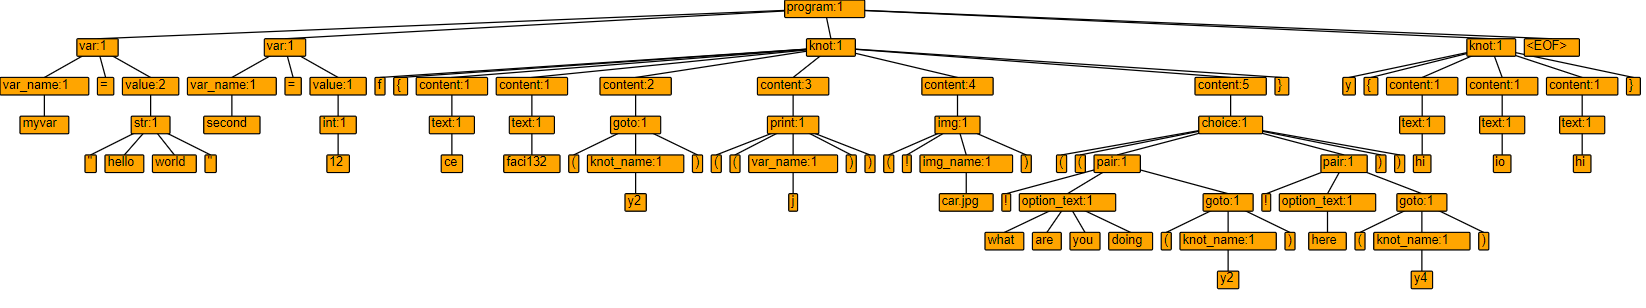
\includegraphics[width=\textwidth]{images/parsetree.png} }


